\documentclass[10pt]{article}
\usepackage{amsmath,amsthm,amssymb,dsfont,graphicx,xspace,epsfig,xcolor}
\usepackage{tikz, tkz-graph, tkz-berge}
\usetikzlibrary{decorations.pathreplacing}
\usetikzlibrary{patterns}
\usetikzlibrary{patterns.meta}
\usepackage{color}

\begin{document}

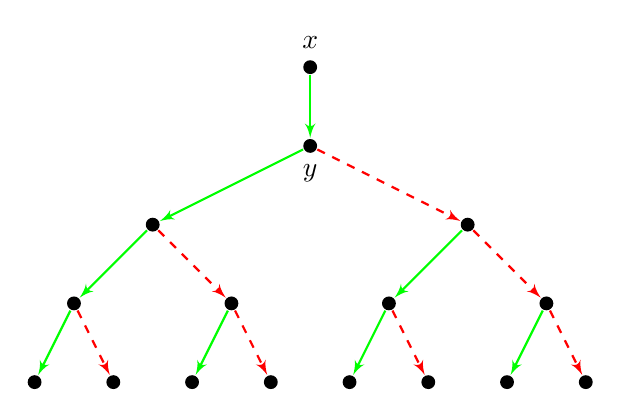
\begin{tikzpicture}[thick,scale=1, every node/.style={transform shape}]
        \tikzset{vertex/.style = {circle,fill=black,minimum size=5pt, inner sep=0pt}}
        \tikzset{littlevertex/.style = {circle,fill=black,minimum size=4pt, inner sep=0pt}}
        \tikzset{edge/.style = {->,> = latex'}}

        \foreach \i in {1,...,4}{
            \pgfmathtruncatemacro{\j}{2*\i - 1}
            \pgfmathtruncatemacro{\k}{2*\i}
            \node[vertex] (a\j) at (\j,0) {};
            \node[vertex] (a\k) at (\k,0) {};
            \node[vertex] (b\i) at (\k-0.5,1) {};
            \draw[edge, green] (b\i) to (a\j){};
            \draw[edge, dashed, red] (b\i) to (a\k) {};
        }
        \node[vertex] (c1) at (2.5,2) {};
        \node[vertex] (c2) at (6.5,2) {};
        \node[vertex, label=below:$y$] (x) at (4.5,3) {};
        \node[vertex, label=above:$x$] (z) at (4.5,4) {};

        \draw[edge, green] (c1) to (b1) {};
        \draw[edge, dashed, red]  (c1) to (b2) {};
        \draw[edge, green] (c2) to (b3){};
        \draw[edge,  dashed, red] (c2) to (b4){};
        \draw[edge, green] (z) to (x) {};
        \draw[edge, green] (x) to (c1) {};
        \draw[edge,  dashed, red] (x) to (c2){};
      \end{tikzpicture}

\end{document}